\chapter[Language fundamentals][Language fundamentals]{Language Fundamentals}\label{chap:language-fundamentals}

In this chapter we define the languages we will study for the remainder of this report. We begin with the language \langrecref{}, defining its syntax, type system and operational semantics. Then we briefly consider a fragment of this language, which we simply call \langpure{}, that we will return to in \cref{chap:logical-predicates,chap:logical-relations}. Next we consider the type system in more detail and describe how to derive new types, as well as how a type system can aid in programming tasks. Finally we prove various properties of the languages' type systems and operational semantics.


\section{The language \texorpdfstring{\langrecref}{F\textunderscore exists,mu,ref}}\index[subject]{Fmuref@\langrecref{}}

The language \langrecref{} is named after Girard's System~$\mathbf{F}$\index[subject]{System $\mathbf{F}$}, which is the simply typed $\lambda$-calculus extended with universal types. In addition, our language has existential types \enquote{$\exists$}, recursive functions and types \enquote{$\mu$}, as well as references \enquote{ref}. The language also has products and sums, but we do not display these in the name of the language to avoid clutter.


\subsection{Syntax}

\newcommand{\setCExp}{\mathit{ClExp}}

We begin by defining the syntax\index[subject]{syntax} of \langrecref{} and describe how the usual representation of such syntax can be understood as defining abstract syntax trees.

As mentioned, \langrecref{} have ASTs of two sorts: expressions and types, denoted $\setExp$\index[notation]{Exp@$\setExp$} and $\setType$\index[notation]{Type@$\setType$} respectively.\blfootnote{We denote by $\setExp$ both the expression sort and the set of ASTs of this sort, and similarly for $\setType$.} The set of \emph{closed} expressions (i.e., expressions with no free variables) is denoted $\setCExp$\index[notation]{ClExp@$\setCExp$}. Furthermore, we divide the set of variables into two infinite sets, one set $\setVar$\index[notation]{Var@$\setVar$} which contains variables of sort $\setExp$, and another set $\setTVar$\index[notation]{TypeVar@$\setTVar$} containing variables of sort $\setType$. Among the operators we have a countably infinite collection $\setLoc$\index[notation]{Loc@$\setLoc$} of nullary operators, which we think of as locations in memory.

The full specification of \langrecref{} is found in \cref{sec:syntax}. For now let us consider only a subset in order to understand how to read this specification:
%
\begin{equation*}
    \begin{array}{lrcl}
            & x,f & \in & \setVar \\
            & l & \in & \setLoc \\
            & \alpha & \in & \setTVar \\
        \setExp 
            & e    & \Coloneqq & \expUnit
                                 \mid x
                                 \mid \expPair{e}{e}
                                 \mid \expRec{f}{x}{e}
                                 \mid \cdots \\
        \setType
            & \tau & \Coloneqq & \typeUnit
                                 \mid \alpha
                                 \mid \typeProd{\tau}{\tau}
                                 \mid \typeFunc{\tau}{\tau}
                                 \mid \cdots
    \end{array}
\end{equation*}
%
The first three lines only serve to introduce notation. The next line defines the operators whose return sort is $\setExp$, with the letter $e$ serving the same role as nonterminal symbols do in formal grammars: For instance, the \enquote{production} $e \Coloneqq \expPair{e}{e}$ says that there is an operator $\expPair{-}{-}$ with arity $\arity{\setExp; \setExp}{\setExp}$. The production $e \Coloneqq x$ simply says that elements of $\setVar$ are expressions\footnote{Strictly speaking this production is redundant, and so is the production $\tau \Coloneqq \alpha$, but we include them to make the specification self-contained.}, and $e \Coloneqq l$ says that locations have return sort $\setExp$. Finally, in the production $e \Coloneqq \expRec{f}{x}{e}$ it is implicit that the variables $f$ and $x$ are bound by the operator in the expression $e$.

Similarly, the next line says, among other things, that there is a nullary operator $\typeUnit$ of sort $\setType$, and that there is an operator $\typeProd{-}{-}$ of arity $\arity{\setType;\setType}{\setType}$.

Notice that operators such as $\expr{rec}$ and $\typ{Ref}$ are written in a sans-serif font, and that the first letter is capitalised when it is an operator whose return sort is $\setType$.


\subsection{Static semantics}\index[subject]{semantics!static}

\subsubsection{Type contexts}

Consider some expression $e$ of \langrecref. If $e$ contains free variables, then in order to decide the type of $e$ we must, at least in the general case, specify types for those variables. We capture this using a \keyword{type context}\index[subject]{type context} which is a finite partial map $\Gamma \colon \setVar \ptofin \setType$. If $\Gamma(x) = \tau$ then we also write $\hastype*{x}{\tau} \in \Gamma$ or just $\hastype{x}{\tau}$\index[notation]{**-colon@$:$ (type of)} when $\Gamma$ is understood.\blfootnote{It is common to define a type context as a finite \emph{list} of pairs $\hastype{x}{\tau}$. Nothing of significance hangs on this for us, but not having to worry about ordering simplifies some proofs.} In this way, $\hastype{x}{\tau}$ also becomes the \emph{assertion} that $x$ has type $\tau$.

If $\Delta$ is another type context such that $\dom \Gamma \intersect \dom \Delta = \emptyset$, then we denote by $\Gamma,\Delta$\index[notation]{gzzzz-GammaDelta@$\Gamma,\Delta$} the type context given by\blfootnote{That is, $\Gamma,\Delta$ is the join $\Gamma \join \Delta$ of the two type contexts in the poset $\pmaps{\setVar}{\setType}$.} % TODO why do we need Gamma and Delta to be disjoint?
%
\begin{equation*}
    (\Gamma,\Delta)(x)
        = \begin{cases}
            \Gamma(x), & x \in \dom\Gamma, \\
            \Delta(x), & x \in \dom\Delta.
        \end{cases}
\end{equation*}
%
Furthermore, if $\dom\Delta = \{x_1, \ldots, x_n\}$ and $\Delta(x_i) = \tau_i$ for distinct $x_i$, then we write $\Gamma, \hastype{x_1}{\tau_1}, \ldots, \hastype{x_n}{\tau_n}$.

We extend the definition of substitution to type contexts: If $\alpha$ is a type variable and $\tau$ a type, then we define
%
\begin{equation*}
    \Gamma[\tau/\alpha](x)
        \defeq \Gamma(x)[\tau/\alpha] \index[notation]{gzzzz-Gammataualpha@$\Gamma[\tau/\alpha]$}
\end{equation*}
%
for all $x \in \dom{\Gamma}$, taking care to rename bound variables as needed. Notice that since $\dom{\Gamma}$ is finite, only finitely many such renamings are necessary.

Similarly, we extend the definition of free type variables to type contexts by letting
%
\begin{equation*}
    \freeTvar{\Gamma}
        \defeq \bigunion_{x \in \dom{\Gamma}} \freeTvar{\Gamma(x)}. \index[notation]{fz-FVTypeGamma@$\freeTvar{}$ (of type context)}
\end{equation*}


\subsubsection{Store typings}

Similarly, the expression $e$ may contain references to locations in memory. A \keyword{store typing}\index[subject]{store typing} is a finite partial map $\Sigma \colon \setLoc \ptofin \setType$ that assigns types to locations. We use the same notation for extending store typings as we did above for type contexts, and substitution\index[notation]{szzzz-Sigmataualpha@$\Sigma[\tau/\alpha]$} and $\freeTvar{\Sigma}$\index[notation]{fz-FVTypeSigma@$\freeTvar{}$ (of store typing)} is defined analogously.


\subsubsection{Free type variables}\label{sec:free-type-var}

Notice that using type contexts we can simultaneously keep track of which variables are (potentially) free in a given expression. In order to get something similar for free \emph{type} variables we may collect the free type variables in a (finite) set $\Xi$ and also keep track of this set. If $\Phi$ is another such set that is disjoint from $\Xi$, then we write\blfootnote{Of course, $\Xi, \Phi$ is the join of $\Xi$ and $\Phi$ in $\powersetfin{\setTVar}$.} $\Xi,\Phi$\index[notation]{xzzzz-XiPhi@$\Xi,\Phi$} for the union $\Xi \union \Phi$. If $\Phi = \{\alpha_1, \ldots, \alpha_n\}$ for distinct $\alpha_i$, then we also write $\Xi, \alpha_1, \ldots, \alpha_n$.

We say that a type $\tau$ is \keyword{well-formed}\index[subject]{type!well-formed} with respect to $\Xi$ if all free type variables in $\tau$ lie in $\Xi$, in which case we write $\wellformed{\Xi}{\tau}$\index[notation]{***-Xitau@$\wellformed{}{}$ (well-formed type)}. If $\Gamma$ is a type context, then we similarly say that $\Gamma$ is well-formed with respect to $\Xi$ if $\wellformed{\Xi}{\tau}$ for all $\tau \in \ran{\Gamma}$, and we also write $\wellformed{\Xi}{\Gamma}$\index[notation]{***-XiGamma@$\wellformed{}{}$ (well-formed type context)}. Well-formedness of store typings with respect to $\Xi$ is defined and denoted analogously.\index[notation]{***-XiSigma@$\wellformed{}{}$ (well-formed store typing)}


\subsubsection{Syntactic typing}

We are now in a position to define the type system for \langrecref{}. This is formalised as a $5$-ary relation on the set
%
\begin{equation*}
    \powersetfin{\setTVar}
        \prod \pmapsfin{\setVar}{\setType}
        \prod \pmapsfin{\setLoc}{\setType}
        \prod \setExp
        \prod \setType
\end{equation*}
%
called the \keyword{syntactic typing relation}\index[subject]{typing relation!syntactic}. Instead of $(\Xi,\Gamma,\Sigma,e,\tau)$, elements of this relation are denoted\blfootnote{The order in which $\Xi$, $\Gamma$ and $\Sigma$ occur is not massively significant. We have chosen this order since it seems the most convenient when we omit one or more of them as noted below.}
%
\begin{equation*}
    \typerel{\Xi}{\Gamma}{\Sigma}{e}{\tau} \index[notation]{***-XiGammaSigmaetau@$\vdash$ (syntactic typing relation)}
\end{equation*}
%
and are called \keyword{typing judgments}\index[subject]{typing judgment}. We also use this notation to assert that this tuple lies in the typing relation. In this case we say that $e$ is \keyword{well-typed}\index[subject]{well-typed} with respect to $\Xi$, $\Gamma$ and $\Sigma$, with type $\tau$. If $\Xi = \emptyset$, then we simply denote the above element by $\typerel{}{\Gamma}{\Sigma}{e}{\tau}$, and we furthermore write $\typerel{}{}{\Sigma}{e}{\tau}$ if also $\Gamma = \bot$. We finally write $\typerel{}{}{}{e}{\tau}$ if also $\Sigma = \bot$, in which case we simply say that $e$ is well-typed.

We define the typing relation using inference rules. As an example, consider the rule\blfootnote{Compare the notation
%
\begin{equation*}
    f : \typeFunc{\tau_1}{\tau_2},
\end{equation*}
%
which says that $f$ is an expression of type $\typeFunc{\tau_1}{\tau_2}$, to the notation
\begin{equation*}
    f \colon \tau_1 \to \tau_2,
\end{equation*}
%
which says that $f$ is an arrow between objects $\tau_1$ and $\tau_2$ of some category. Notice in particular the spacing around the colon \enquote{$:$}.}
%
\begin{equation*}
    \ruleTrec*.
\end{equation*}
%
This says that given an expression $e$ having (potentially) free variables $f$ and $x$ of appropriate types, we may construct an expression $\expRec{f}{x}{e}$ of function type, whose parameter type is that of $x$, and whose return type is the return type of $f$. Note that the store typing $\Sigma$ and the set $\Xi$ of free type variables are unchanged when moving from the premise to the conclusion, while the variables $f$ and $x$ are no longer assigned types by the type context in the conclusion.

Consider instead the rule
%
\begin{equation*}
    \ruleTvar*
\end{equation*}
%
which assigns types to variables. This rule is not quite on the correct form, since its hypotheses are not elements of the typing relation. The intended interpretation is that given the assumptions $\wellformed{\Xi}{\Gamma}$, $\wellformed{\Xi}{\Sigma}$ and $\Gamma(x) = \tau$ we have the rule (in fact the axiom)
%
\begin{equation*}
    \inferrule{ }{
        \typerel{\Xi}{\Gamma}{\Sigma}{x}{\tau}
    }.
\end{equation*}


\subsection{Dynamic semantics}\label{sec:dynamic-semantics}

The last piece of the definition of \langrecref{} is its dynamic semantics\index[subject]{semantics!dynamic}. We specify an operational (transition) semantics\index[subject]{semantics!operational}\index[subject]{semantics!transition} in several steps.

The resulting dynamics consists of performing reductions at three different levels:
%
\begin{itemize}
    \item The first level consists of \emph{pure head reductions}. These are reductions that can be performed on expressions that have no subexpressions that can be evaluated, and without reading or modifying the store\footnote{We describe what we mean by \enquote{store} in more detail below.}.
    
    \item The next level are the \emph{impure} head reductions. Here we again reduce simple expressions, but these may read from or write to the store.

    \item The final level allows us to perform reductions on complex expressions by reducing subexpressions.
\end{itemize}
%
At each level we define a transition system on machine states using inference rules.


\subsubsection{Pure head reductions}\label{sec:pure-head-red}\index[subject]{reduction!pure head}

\newcommand{\setIrr}{\mathit{Irr}}

As mentioned, we do not yet wish to reduce complex expressions, so we need to make precise what we mean by a \enquote{simple} expression. We call an expression a \keyword{value} if it is to be considered the final result of a computation. We define the set $\setVal$ of values recursively:
%
\begin{equation*}
    v \Coloneqq \expUnit \mid l \mid \expPair{v}{v} \mid \cdots
\end{equation*}
%
We use the letter \enquote{$v$}, often with various decorations, to denote values. The set of \emph{closed} values (i.e., values with no free variables) will be denoted $\setCVal$\index[notation]{ClVal@$\setCVal$}. Furthermore, as the end result of computations, values are naturally supposed to be irreducible, and indeed they turn out to be (cf. \cref{prop:value-implies-irreducible}). We denote the set of irreducible expressions by $\setIrr$.\index[notation]{Irr@$\setIrr$}

Furthermore, when performing pure reductions we do not need to take into account memory, so we simply model the machine state\index[subject]{machine state} by a single expression. The pure head reduction, which we denote by $\purestep$\index[notation]{***-steppure@$\purestep$}, is thus a binary relation on $\setExp$.

As an example of a pure reduction rule, consider the rule
%
\begin{equation*}
    \ruleEprojl*.
\end{equation*}
%
Since both $v_1$ and $v_2$ are values, these are not supposed to be reduced further, so the expression $\expProjl{\expPair{v_1}{v_2}}$ has no reducible subexpressions.


\subsubsection{Impure head reductions}\label{sec:impure-head-reduction}\index[subject]{reduction!impure head}

Next we must take into account mutable state. We model memory access using a \keyword{store}\index[subject]{store}\blfootnote{Some authors use the word \keyword{heap}\index[subject]{heap|see{store}} instead of store, which is not to be confused with the heap data structure.}, which is a finite partial map $\sigma \colon \setLoc \ptofin \setExp$. Denote by $\setSto$\index[notation]{Sto@$\setSto$} the set of stores. We thus model machine states\index[subject]{machine state} as elements of the product $\setSto \prod \setExp$, and the impure head reduction, denoted $\headstep$\index[notation]{***-stephead@$\headstep$}, becomes a binary relation on this product.

All pure head reductions give rise to impure head reductions: We formalise this by adding a rule
%
\begin{equation*}
    \ruleEpure*
\end{equation*}
%
for every store $\sigma$. To take an example of a rule that modifies the store, consider
%
\begin{equation*}
    \ruleEalloc*.
\end{equation*}
%
This rule allows us to place the value $v$ in the store by wrapping it in a $\expr{ref}$ expression and evaluating it. Note that this rule is non-deterministic, since the location $l$ is not uniquely specified by the hypothesis: Indeed, since the domain of a store is finite but the set $\setLoc$ of locations is infinite, the value $v$ could be saved at an infinite number of locations. For our purposes we could have modified the rule \ruleref{Ealloc} to be deterministic, for instance by enumerating the locations and always allocating the location that is smallest with respect to this enumeration. However, in practice memory allocation is (partially) handled by the operating system and is not deterministic\footnote{At least from the point of view of the programmer.}, so we prefer the the non-deterministic version.


\subsubsection{Evaluation contexts}\label{sec:evaluation-contexts}

In order to reduce a complex expression $e$, we must somehow locate a simple subexpression of $e$ that can be reduced directly. Furthermore, there may be multiple such subexpressions, so we must also decide in which order these should be reduced. We do this by introducing \keyword{evaluation contexts}\index[subject]{context!evaluation}\index[subject]{evaluation context|see{context, evaluation}}: Recall that we in \cref{sec:reduction-in-ASTs} introduced \emph{contexts} which are, roughly speaking, expressions in which one subexpression has been replaced by the hole $\hole$. A subset of these will serve as evaluation contexts, namely those given by the following recursive definition:\blfootnote{Again the complete specification can be found in \cref{sec:syntax}.}
%
\begin{equation*}
    E \Coloneqq \hole \mid \expPair{E}{e} \mid \expPair{v}{E} \mid \cdots
\end{equation*}
%
As before, $e$ denotes an expression and $v$ a value. We collect the evaluation contexts in a set $\setECtx$\index[notation]{ECtx@$\setECtx$}.

Recall also that contexts are in general \emph{capturing}, in that the expression $e$ may contain free variables that are captured by bindings in a context $C$ when inserting $e$ into $C$. But notice that this is not the case for evaluation contexts. This for instance means that the body of a function is not evaluated before the function has been applied to an argument.

This also means that there is another way to define evaluation contexts: We could backtrack and add the hole to our initial specification of \langrecref{}. In this case the hole cannot be an expression, since this would allow undesirable expressions such as $\expPair{\hole}{\hole}$. We could instead let $\setECtx$ be its own sort, but then for $\expPair{E}{e}$ to be an evaluation context the pairing operator must have three different arities, namely $\arity{\setExp;\setExp}{\setExp}$, $\arity{\setECtx;\setExp}{\setECtx}$ and $\arity{\setExp;\setECtx}{\setECtx}$. If we assign each operator multiple different arities, and if we furthermore let the hole be a \emph{variable}, then one can show that substituting an expression into the hole does indeed yield an expression. Furthermore, one can show that we have $E[e/\hole] = E[e]$. No matter which definition we use, each $E$ gives rise to a map $\setExp \to \setExp$ given by $e \mapsto E[e]$. % TODO write something about substitution vs replacement

We can now define the final transition system that formalises the operational semantics of \langrecref{}. The reduction $\step$\index[notation]{***-step@$\step$} is defined by the single rule schema
%
\begin{equation*}
    \ruleEhead*.
\end{equation*}
%
Notice that this is \emph{almost} the consistent closure of $\headstep$, except that we also need to keep track of stores.


\section{The language fragment \langpure}\index[subject]{F@\langpure{}}\label{sec:langpure}

In addition to the \enquote{full} language \langrecref{} we will also have reason to study a fragment that has neither recursive types nor references, which we call \langpure{}. To further simplify we also omit existential types.

Since \langpure{} does not have references, we have no need to keep track of a store. Hence we agree that when studying this language, we model the machine state using only an expression, and we thus omit the store from our notation.

We return to this language in \cref{cor:determinism-multistep}, and in \cref{chap:logical-predicates,chap:logical-relations} it will be our main focus, but until then all references are to \langrecref{} unless otherwise specified.


\section{Programming with types}

In this section we consider each of the types of \langrecref{} and discuss in greater or lesser detail what each type can be used for in practice.


\subsection{Base types}

\newcommand{\typeNat}{\typ{Nat}}
\newcommand{\expZero}{\expr{0}}
\newcommand{\expSucc}[1]{\expr{succ}\expspace#1}
\newcommand{\expTuple}[1]{\langle#1\rangle}

The only \keyword{base type}\index[subject]{type!base} in \langrecref{} is the unit type\index[subject]{type!unit} $\typeUnit$\index[notation]{01-typeunit@$\typeUnit$ (unit type)} whose only value is\footnote{This fact will follow from \cref{enum:canonical-unit}.} $\expUnit$\index[subject]{expression!unit}\index[notation]{01-valunit@$\expUnit$ (unit value)}. This is used for various purposes: to indicate the absense of a value, as a \enquote{sentinel value}\index[subject]{sentinel value}, or as the value of expressions that are only used for their side effects.

Since the unit type categorically is an empty product, hence a terminal object, we denote the type by $\typeUnit$. We could have denoted the unit \emph{value} by $\langle\rangle$ to represent an empty tuple, but we prefer $\expUnit$ for purely aesthetic reasons. No confusion is likely to result from this choice.

Other common base types are booleans, numbers and strings. We construct booleans in \cref{sec:booleans} below, and in \cref{sec:existential-types} we will also consider a base type $\typeNat$ of natural numbers\index[subject]{type!natural numbers} for expository purposes.

Sometimes \keyword{uninterpreted}\index[subject]{type!uninterpreted base} base types \textdash i.e., base types that have no constructors or eliminators \textdash are also used. Type variables can be considered to be of this sort\footnote{See \textcite[§22.1]{pierce-types}. Though note that for us variables are by definition different from operators with the same sort.}.


\subsection{Products and sums}

The product\index[subject]{type!product} $\typeProd{\tau_1}{\tau_2}$\index[notation]{****-typeprod@$\prod$ (product type)} of types $\tau_1$ and $\tau_2$ should be well-known: It is simply the type of pairs\index[subject]{expression!pair} $\expPair{e_1}{e_2}$\index[notation]{****-exppair@$\expPair{\blank}{\blank}$} of expressions, where $e_i$ has type $\tau_i$.

The sum\index[subject]{type!sum} $\typeSum{\tau_1}{\tau_2}$\index[notation]{****-typesum@$+$ (sum type)} is perhaps less familiar. Its values are \emph{either} of type $\tau_1$ \emph{or} of type $\tau_2$, and each value of type $\typeSum{\tau_1}{\tau_2}$ is decorated to indicate which type it belongs to. Thus the sum is effectively the disjoint union\footnote{Indeed, it is possible to construct a category of types\index[subject]{category of types} in which products are categorical products and sums are categorical coproducts, i.e., analogous to disjoint unions in the category of sets. For a brief description of such a category see \textcite[§2.5]{awodey-category-theory}.} of $\tau_1$ and $\tau_2$. If $e_1$ and $e_2$ are expressions of types $\tau_1$ and $\tau_2$, then we denote by $\expInjl{e_1}$\index[notation]{izzzz-inj1e@$\iota_1$} and $\expInjr{e_2}$\index[notation]{izzzz-inj2@$\iota_2$} their injections\index[subject]{expression!injection} into the type $\typeSum{\tau_1}{\tau_2}$.

We will see applications of both products and sums below.


\subsection{Booleans}\label{sec:booleans}

A boolean\index[subject]{type!boolean} type is nothing but a type with two values.\blfootnote{Our definition of $\expFalse$ and $\expTrue$ require us to change the ordering of the expressions $e_1$ and $e_2$ in the match expression below. This slightly inconvenient choice arises from interpreting the type $\typeUnit$ as the singleton $\{\expUnit\}$ with the trivial ordering and the sum $\typeSum{\typeUnit}{\typeUnit}$ as the \emph{linear} sum of its summands, meaning as the disjoint union equipped with the ordering $\expInjl{\expUnit} < \expInjr{\expUnit}$. Interpreting the smaller of these as false corresponds to interpreting the ordering as logical implication. \par This is consistent with the convention that $0$ represents false and $1$ true given the ordering $0 < 1$.} Instead of \enquote{hard-coding} booleans into \langrecref{}, we may construct such a type using sum types: We can simply use $\typeSum{\typeUnit}{\typeUnit}$ whose values are of course $\expInjl{\expUnit}$ and $\expInjr{\expUnit}$. We use $\typeBool$\index[notation]{Bool@$\typeBool$} as an alias for this sum type, and $\expFalse$\index[notation]{false@$\expFalse$} and $\expTrue$\index[notation]{true@$\expTrue$} as aliases for its values, respectively.

To implement an if-expression we define the expression
%
\begin{equation*}
    \expIf{e}{e_1}{e_2} \index[notation]{ifthenelse@$\expIf{e}{e_1}{e_2}$}
\end{equation*}
%
as syntactic sugar for $\expMatch{e}{x}{e_2}{e_1}$, where $x$ is a variable that is not free in either $e_1$ or $e_2$. In particular we have, by \ruleref{Ematchinjl},
%
\begin{align*}
    \expIf{\expFalse}{e_1}{e_2}
        &= \expMatch{\expInjl{\expUnit}}{x}{e_2}{e_1} \\
        &\purestep e_2[\expUnit/x] \\
        &= e_2,
\end{align*}
%
and \ruleref{Ematchinjr} similarly implies that $\expIf{\expTrue}{e_1}{e_2} \purestep e_1$.

We furthermore obtain the evaluation contexts
%
\begin{equation*}
    E
        \Coloneqq \cdots \mid \expIf{E}{e}{e},
\end{equation*}
%
showing that we may evaluate the condition but neither of the branches, as expected.


\subsection{Options}

Sum\blfootnote{\enquote{Option} is the name given to these types in languages such as ML or Coq, while e.g. Haskell or Agda call them \enquote{maybe} types.} types also allow us to implement option types\index[subject]{type!option}. Given a type $\tau$ we construct a type that can contain either \enquote{nothing} or an expression of type $\tau$. We use the type $\typeUnit$ to model the first case, and we collect the types in the sum $\typeSum{\typeUnit}{\tau}$. Let $\typeOpt{\tau}$\index[notation]{oz-opttau@$\typeOpt{\tau}$} be an alias for this type.

As \enquote{value constructors} we define $\expNothing = \expInjl{\expUnit}$\index[notation]{none@$\expNothing$} and $\expJust{e} = \expInjr{e}$\index[notation]{just@$\expJust{e}$}. We can also introduce syntactic sugar for pattern matching on options:
%
\begin{equation*}
    \expWhich{e}{x}{e_1}{e_2}
        = \expMatch{e}{x}{e_1}{e_2}. \index[notation]{which@$\expr{which}$}
\end{equation*}
%
If $e$ is $\expNothing$ this reduces to $e_1[\expUnit/x]$, and it reduces to $e_2[e'/x]$ otherwise where $e = \expJust{e'}$. Notice that this allows $x$ to also be free in $e_1$, which is probably not the intended behaviour. Notice also that if we implement options and booleans simultaneously, then $\expFalse$ and $\expNothing$ are aliases for the same value, which is also probably undesirable.

Option types can also be implemented using labeled sums, so-called \keyword{variants}\index[subject]{type!variant} (cf. \cite[§11.10]{pierce-types}), in which option types and $\typeBool$ can be made disjoint, though a programmer can of course still unintentionally construct values of option type.


\subsection{An empty type}

If\blfootnote{In fact, universal types are so expressive that we can even use them to implement products and sums, cf. \textcite[§16.2]{harper-pl}.} no expressions has a type $\tau$, then $\tau$ is an empty\index[subject]{type!empty|see{type, void}} or \keyword{void} type\index[subject]{type!void}. We can implement such a type as $\typeForall{\alpha}{\alpha}$.

Note that the terminology surrounding empty and unit types is not exactly standardised. For instance, the type \texttt{Void} in Java is in fact a unit type, since its only value is \texttt{null}. On the other hand, the type \texttt{void} in C seems to occupy a role somewhere in between: While no object has type \texttt{void}, functions whose return type is \texttt{void} can in fact terminate.


\subsection{Polymorphic types}\label{sec:programming-polymorphism}\index[subject]{type!polymorphic}\index[subject]{polymorphism|see{type, polymorphic}}

\subsubsection{Universal types}\label[subject]{type!universal}

\newcommand{\expDouble}{\expr{double}}
\newcommand{\expNeg}{\expr{neg}}
\newcommand{\expId}{\expr{id}}

Universal types should be familiar to anyone experienced with functional programming, though perhaps in a different guise. We attempt to motivate universal types using a simplified version of a classic example.

Let\blfootnote{This example is based on \textcite[§22.7]{pierce-types}. Notice that the language studied by \citeauthor{pierce-types} has type annotations and let-expressions; we emulate the latter using lambdas (and products), and the former turns out not to make a difference for our purposes.} $\expId = \expLam{x}{x}$\index[notation]{id@$\expId$} be the identity function.\index[subject]{function!identity} The expression
%
\begin{equation*}
    \expPair{
        \expApp{
            \expId
        }{
            \expTrue
        }
    }{
        \expApp{
            \expId
        }{
            \expUnit
        }
    }
\end{equation*}
%
is then completely unproblematic: Even though the expression $\expId$ appears in both entries in the pair applied to expressions of different types, the two occurrences of $\expId$ are simply assigned different types. But a problem arises when we factor $\expId$ out as follows:
%
\begin{equation}
    \label{eq:polymorphism-example}
    \expApp{
        \expLam*{f}{
            \expPair{
                \expApp{
                    f
                }{
                    \expTrue
                }
            }{
                \expApp{
                    f
                }{
                    \expUnit
                }
            }
        }
    }{
        \expId
    }.
\end{equation}
%
The inversion lemma (which we will meet in \cref{lem:inversion-typing}) implies that if $\expId$ has type $\rho$, then
%
\begin{equation*}
    f : \rho \vdash
    \expPair{
        \expApp{
            f
        }{
            \expTrue
        }
    }{
        \expApp{
            f
        }{
            \expUnit
        }
    }
    : \tau
\end{equation*}
%
for some type $\tau$, which must be on the form $\typeProd{\tau_1}{\tau_2}$. Further application of the inversion lemma then shows that
%
\begin{equation*}
    f : \rho \vdash
        f : \typeFunc{\typeBool}{\tau_1}
\end{equation*}
%
and
%
\begin{equation*}
    f : \rho \vdash
        f : \typeFunc{\typeUnit}{\tau_2}
\end{equation*}
%
simultaneously. But then we must have\footnote{Notice that this argument does not appeal to \emph{uniqueness} of types, but simply uses the inversion lemma. We return to the question of uniqueness in \cref{sec:type-uniqueness}.}
%
\begin{equation*}
    \typeFunc{\typeBool}{\tau_1}
        = \rho
        = \typeFunc{\typeUnit}{\tau_2},
\end{equation*}
%
which is impossible since $\typeBool$ and $\typeUnit$ are distinct types.

However, it seems like we morally should be able to write something like \cref{eq:polymorphism-example}. Clearly the function $\expId$ does not care about the type of its argument, and in many languages without static type checking we could easily get away with such an expression.

We solve this problem as follows: Instead of requiring that the types of expressions be closed, we allow them to contain type variables. Just as with expression variables, we then introduce \emph{abstractions} on type variables, lambda expressions that take types instead of expressions as arguments. To distinguish these from ordinary lambda expressions, we use a capital $\Lambda$. If $e$ is an expression whose type $\tau$ may contain type variables, among these $\alpha$, we can then write\footnote{This is not our official syntax since this does not contain explicit type variables. We return to this below.} $\Lambda \alpha . e$ to denote an expression which takes a type $\tau'$ as argument and yields an expression with type $\tau[\tau'/\alpha]$. The expression $\Lambda \alpha . e$ then becomes polymorphic in the sense that we may instantiate $\alpha$ in $\tau$ as any type, though note that if $\tau$ has no other free type variables than $\alpha$, then the type of $\Lambda \alpha . e$ is closed. We denote the type of $\Lambda \alpha . e$ by $\typeForall{\alpha}{\tau}$.

For instance, we can define a polymorphic version of the identity function\index[subject]{function!polymorphic identity} as follows: The expression $\expLam{x}{x}$ has type $\typeFunc*{\alpha}{\alpha}$, where $\alpha$ is a type variable, so the expression
%
\begin{equation*}
    \expId
        = \Lambda \alpha . \expLam{x}{x}
\end{equation*}
%
then has type $\typeForall{\alpha}{\typeFunc*{\alpha}{\alpha}}$. To instantiate $\alpha$ as a concrete type, say $\typeBool$, we write\footnote{Again our official syntax does not use explicit types in expressions.} $\expApp{\expId}{[\typeBool]}$. Returning to the untypable expression in \cref{eq:polymorphism-example}, by using the polymorphic version of $\expId$ we can write
%
\begin{equation*}
    \expApp{
        \expLam*{f}{
            \expPair{
                \expApp{
                    \expApp{f}{[\typeBool]}
                }{
                    \expTrue
                }
            }{
                \expApp{
                    \expApp{f}{[\typeUnit]}
                }{
                    \expUnit
                }
            }
        }
    }{
        \expId
    },
\end{equation*}
%
which is then well-typed.

\newcommand{\typeList}[1][]{%
    \ifstrempty{#1}{%
        \typ{List}%
    }{%
        #1\text{-}\typ{List}%
    }%
}

The above example is fairly artificial, but parametric polymorphism is of course ubiquitous in functional programming: For a simple example, lists are usually polymorphic in the sense that to each type $\tau$ there is a type of $\tau$-lists where expressions of such a type are lists whose elements all are of type $\tau$. Using the recursive list type $\typeList[\tau] = \typeRec{\alpha}{\typeSum{\typeUnit}{\typeProd*{\tau}{\alpha}}}$ we will construct in \cref{sec:recursive-types}, we obtain a polymorphic list type\index[subject]{type!polymorphic list} by
%
\begin{equation*}
    \typeList
        \defeq \typeForall{\beta}{\typeRec{\alpha}{\typeSum{\typeUnit}{\typeProd*{\beta}{\alpha}}}}. \index[notation]{lz-list@$\typeList$}
\end{equation*}

Finally we note that \langrecref{} does not have explicit types. Instead of $\Lambda \alpha . e$ we replace the type variable with a wildcard and write $\expForall{\alpha}{e}$, and instead of $\expApp{e}{[\tau]}$ we similarly write $\expTapp{e}{\tau}$. This of course makes the type checker's job more difficult, but this is not a concern for us in this report.


\subsubsection{Existential types}\label{sec:existential-types}\index[subject]{type!existential}

\newcommand{\expPackAs}[4]{\expr{pack}\expspace(#1,#2)\expspace\expr{as}\expspace\typeExists{#3}{#4}}

Since\blfootnote{In fact, existential types can be encoded using universal types, cf. \textcite[§24.3]{pierce-types}.} we can universally quantify over type variables, it seems reasonable to assume that we can also \emph{existentially} quantify over them.

If an expression has the existential type $\typeExists{\alpha}{\tau}$, then this supposedly means that there is some type $\tau'$ such that the expression has type $\tau[\tau'/\alpha]$. Notice that there might be multiple different types $\tau'$ such that $e$ has type $\tau[\tau'/\alpha]$: For instance, if $e$ is the expression $\expLam{x}{\expUnit}$, then this has type $\typeFunc{\tau'}{\typeUnit}$ for any type $\tau'$. When we abstract away this type $\tau'$, it is therefore useful to keep track of it. If an expression $e$ has type $\tau[\tau'/\alpha]$, then we therefore (tentatively) introduce an expression of existential type $\typeExists{\alpha}{\tau}$ by\footnote{The name \enquote{pack} will make sense shortly. As for universal types this notation is temporary, and we introduce our official notation below.} $\expPack{(e,\tau')}$\index[notation]{pack2@$\expr{pack}$}. We keep track of the \keyword{witness type}\index[subject]{type!witness} $\tau'$, but notice that this does not appear in the existential type itself, meaning that it cannot be used to typecheck. We therefore also call it the \keyword{hidden representation type}\index[subject]{type!hidden representation}.

Furthermore, the expression $\expPack{(\expLam{x}{\expUnit},\tau')}$ itself also has multiple types, for instance $\typeExists{\alpha}{\typeFunc{\typeUnit}{\typeUnit}}$ and even $\typeExists{\alpha}{\typeFunc{\alpha}{\alpha}}$. Hence it is also useful when introducing an expression of either type to specify which type it should be introduced as, and so we might write something like\blfootnote{Notice that the \enquote{as}-clause is a kind of \keyword{ascription}\index[subject]{ascription}, cf. \textcite[§11.4]{pierce-types}.}
%
\begin{equation*}
    \expPackAs{\expLam{x}{\expUnit}}{\tau'}{\alpha}{\typeFunc{\alpha}{\alpha}}. % \index[notation]{packas@$\expr{packas}$}
\end{equation*}

Existential types can be used as a sort of primitive module system by allowing us to implement abstract data types. Under this interpretation we also think of expressions of existential type as \emph{packages}. As an example, we implement an abstract counter type\footnote{This example is adapted from \textcite[§24.2]{pierce-types}.}.\index[subject]{type!counter} Assuming that we have a natural number type\index[subject]{type!natural numbers} $\typeNat$\index[notation]{nz-Nat@$\typeNat$}, a constructor $\expZero$\index[notation]{00-0@$\expZero$ (zero value)} and a successor operation $\expr{succ}$\index[notation]{succ@$\expr{succ}$}, we use $\typeNat$ as the hidden representation type. Since this is not available to the user, this allows us as \enquote{maintainers} of this package to change the internal representation without issue.

The counter type should be able to create new counters, increment counters, and return the value of a counter. Creating a new counter is simple, we just use the constructor $\expZero$. To increment a counter we can use the function $\expLam{n}{\expSucc{n}}$, and to return its value we simply return the natural number used internally, so we use the identity function $\expLam{n}{n}$. In total the internal representation of the type becomes\blfootnote{We here use a tuple with three elements to simplify notation, but this can of course be implemented as two nested pairs.}
%
\begin{equation*}
    \expTuple{
        \expZero,
        \expLam{n}{\expSucc{n}},
        \expLam{n}{n}
    },
\end{equation*}
%
and when packed with representation type $\typeNat$ it receives the existential type
%
\begin{equation*}
    \typeExists{\alpha}{
        \typeProd*{
            \typeProd{\alpha}{\typeFunc*{\alpha}{\alpha}}
        }{
            \typeFunc*{\alpha}{\typeNat}
        }
    }.
\end{equation*}
%
That is, we obtain the expression
%
\begin{equation*}
    \expPackAs{
        \expTuple{
            \expZero,
            \expLam{n}{\expSucc{n}},
            \expLam{n}{n}
        }
    }{
        \typeNat
    }{
        \alpha
    }{
        \typeProd*{
            \typeProd{\alpha}{\typeFunc*{\alpha}{\alpha}}
        }{
            \typeFunc*{\alpha}{\typeNat}
        }
    }.
\end{equation*}
%
This is the expression that is available to users of the package, and notice again that while the hidden representation type $\typeNat$ does appear in the expression, it is not part of the type and so does not affect type checking.

\newcommand{\expUnpackAs}[4]{\expr{unpack}\expspace#1\expspace\expr{as}\expspace(#2,#3)\expspace\expr{in}\expspace#4}

We also need a way to \enquote{unpack} packages. Given a package $p$ of type $\typeExists{\alpha}{\tau}$, we need some way of \enquote{importing} $p$ and extracting its components. Say that $e$ is the program in which we wish to use $p$, and that we wish to bind the contents of $p$ to a variable $x$. Then $x$ must have the correct type, namely $\tau$ (perhaps containing the type variable $\alpha$). The hidden representation type of $p$ will also become bound to $\alpha$ in $e$ if it occurs free. We may write this as follows:
%
\begin{equation*}
    \expUnpackAs{p}{x}{\alpha}{e}. % \index[notation]{unpackas@$\expUnpackAs{p}{x}{\alpha}{e}$}
\end{equation*}
%
More explicitly, say that $p$ is the expression $\expPackAs{v}{\tau'}{\alpha}{\tau}$, where $v$ is a value. We then reduce the above expression as
%
\begin{equation*}
    \expUnpackAs{
        (\expPackAs{v}{\tau'}{\alpha}{\tau})
    }{x}{\alpha}{e}
        \purestep e[v/x][\tau'/\alpha].
\end{equation*}
%
Note that \langrecref{} does not have explicit types, so we simplify the pack-unpack notation and instead simply write $\expPack{v}$ and $\expUnpack{p}{x}{e}$.


\subsection{Recursive types}\label{sec:recursive-types}\label{type!recursive}

A recursive type is, roughly speaking, a type that is defined in terms of itself, or properly contains itself syntactically\footnote{That is, it is a proper \enquote{subtype} of itself in the sense of sub-ASTs, not in the usual sense of subtyping.}. In a sense a recursive type is thus somehow infinite, so to properly understand recursive types, we begin by considering how types can be represented as various kinds of objects that can be either finite or infinite.

Types can of course be represented using potentially infinite strings, but they are more naturally represented by rooted trees\index[subject]{type!tree}; almost obviously, since we have even defined them as abstract syntax \emph{trees}. This representation is of course very natural: The leaves are either base types or type variables, and the inner vertices are operators whose children are their arguments. An example is given in \cref{fig:tree-type-finite}.

\begin{marginfigure}\small
    \begin{tikzpicture}[scale=0.5,xscale=0.7]
        \node (root) at (0,0) {$\typeSum{}{}$};
        \node (1left) at (-2,-2) {$\typeUnit$};
        \node (1right) at (2,-2) {$\typeProd{}{}$};
        \node (2left) at (0,-4) {$\typeUnit$};
        \node (2right) at (4,-4) {$\alpha$};
        \draw (root) -- (1left);
        \draw (root) -- (1right) -- (2left);
        \draw (1right) -- (2right);
    \end{tikzpicture}
    \caption{Tree representing the type $\protect\typeSum{\typeUnit}{\protect\typeProd*{\typeUnit}{\alpha}}$.}
    \label{fig:tree-type-finite}
\end{marginfigure}

\begin{marginfigure}\small
    \begin{tikzpicture}[scale=0.5,xscale=0.7]
        \node (root) at (0,0) {$\typeFunc{}{}$};
        \node (1left) at (-2,-2) {$\typeUnit$};
        \node (1right) at (2,-2) {$\typeFunc{}{}$};
        \node (2left) at (0,-4) {$\typeUnit$};
        \node (2right) at (4,-4) {$\typeFunc{}{}$};
        \node (3left) at (2,-6) {$\typeUnit$};
        \node (3right) at (6,-6) {};
        \draw (root) -- (1right) -- (2right);
        \draw (2right)[dash pattern=on 8pt off 2pt on 2pt off 2pt on 2pt off 2pt on 2pt off 2pt on 2pt off 2pt] -- (3right); % TODO copy this pattern to appendix as well
        \draw (root) -- (1left);
        \draw (1right) -- (2left);
        \draw (2right) -- (3left);
    \end{tikzpicture}
    \caption{An infinite tree representing the \enquote{infinite type} $\protect\typeFunc{\typeUnit}{\protect\typeFunc*{\typeUnit}{\protect\typeFunc*{\typeUnit}{\cdots}}}$.}
    \label{fig:tree-type-infinite}
\end{marginfigure}

% TODO make a typeFuncOp etc.

In the other direction we can imagine \emph{infinite} trees that have the same general structure: Leaves are still base types or type variables, inner vertices are operators with the correct number of children, but the tree is infinite. For instance, consider the tree in \cref{fig:tree-type-infinite}. The outermost operator (i.e., the root of the tree) is $\typeFunc{}{}$, so if this tree is supposed to represent a type, then it must be a function type. The argument type is $\typeUnit$, but notice that the right child of the root is just another copy of the whole tree. Apparently, an expression of this type is a function that takes $\expUnit$ as an argument and returns a function of the same type as itself. If $\tau$ denotes (the type represented by) the whole tree, we thus have $\tau = \typeFunc{\typeUnit}{\tau}$. We denote $\tau$ by $\typeRec{\alpha}{\typeFunc{\typeUnit}{\alpha}}$, motivated by the fact that $\tau$ is a fixed-point of the map $\alpha \mapsto \typeFunc{\typeUnit}{\alpha}$.

For a more immediately useful example, we show how to construct a recursive list type\index[subject]{type!list}: Recall that in order to construct a linked list, we need a \enquote{nil}\index[subject]{nil} object to represent the empty list and a \enquote{cons}\enquote{nil}\index[subject]{cons} operation that pairs two objects. If we use $\expUnit$ to represent the empty list and the built-in pairs $\expPair{\hole}{\hole}$ for pairing, then an informal specification of a type $\typeList[\tau]$ of lists of elements of type $\tau$ could look like
%
\begin{equation*}
    \typeList[\tau]
        \Coloneqq \expUnit \mid \expPair{\tau}{\typeList[\tau]}.
\end{equation*}
%
More precisely, we would have $\typeList[\tau] = \typeRec{\alpha}{\typeSum{\typeUnit}{\typeProd*{\tau}{\alpha}}}$.

What we have outlined is the \keyword{equi-recursive}\index[subject]{equi-recursive} approach to recursive types, in which the recursive type $\tau$ is by definition \emph{equal} to its \enquote{unfolded} counterpart $\typeFunc{\typeUnit}{\tau}$. More generally, a recursive type $\typeRec{\alpha}{\tau}$ is equal to the type $\tau[\typeRec{\alpha}{\tau}/\alpha]$. An alternative is the \keyword{iso-recursive}\index[subject]{iso-recursive} approach, in which the types $\typeRec{\alpha}{\tau}$ and $\tau[\typeRec{\alpha}{\tau}/\alpha]$ are seen as different but somehow \emph{isomorphic}. The isomorphism is witnessed by maps $\expr{unfold}$ and $\expr{fold}$ that yield a correspondence between expressions of the two types, as schematically presented in \cref{fig:unfold-fold}.

\begin{marginfigure}\small
    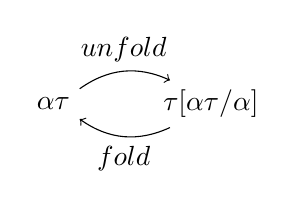
\begin{tikzpicture}[scale=0.5]
        \node (folded) at (0,0) {$\typeRec{\alpha}{\tau}$};
        \node (unfolded) at (4,0) {$\tau[\typeRec{\alpha}{\tau}/\alpha]$};
        \draw[->,bend left] (folded) to node[above] {$\expr{unfold}$} (unfolded);
        \draw[->,bend left] (unfolded) to node[below] {$\expr{fold}$} (folded);
    \end{tikzpicture}
    \caption{Correspondence between a recursive type $\protect\typeRec{\alpha}{\tau}$ and its \enquote{unfolded} version $\tau[\protect\typeRec{\alpha}{\tau}/\alpha]$.}
    \label{fig:unfold-fold}
\end{marginfigure}

\newcommand{\expNil}{\expr{nil}}
\newcommand{\expCons}{\expr{cons}}

We construct a recursive list type. Let $\tau$ be the type of the elements of the list, and assume that $\alpha$ is not free in $\tau$. The expression $\expInjl{\expUnit}$ has type $\typeSum{\typeUnit}{\typeProd*{\tau}{\typeList[\tau]}}$, so we fold it and obtain the expression $\expNil \defeq \expFold{\expInjl{\expUnit}}$\index[notation]{nil@$\expNil$} with type $\typeList[\tau] = \typeRec{\alpha}{\typeSum{\typeUnit}{\typeProd*{\tau}{\alpha}}}$. We similarly want a cons operator, and this should take an expression of type $\tau$ and prepend this to a $\tau$-list, so it should be of type $\typeFunc{\tau}{\typeFunc{\typeList[\tau]}{\typeList[\tau]}}$. Given expressions $x$ and $l$ of type $\tau$ and $\typeList[\tau]$ respectively, the expression $\expInjr{\expPair{x}{l}}$ has type $\typeSum{\typeUnit}{\typeProd*{\tau}{\typeList[\tau]}}$, so folding this and abstracting out $x$ and $l$ we obtain
%
\begin{equation*}
    \expCons
        \defeq \expLam{x}{\expLam{l}{\expFold{\expInjr{\expPair{x}{l}}}}} \index[notation]{cons@$\expCons$}
\end{equation*}
%
with the correct type.

In order to use expressions with recursive types we first reduce the argument to $\expr{fold}$ to a value and apply $\expr{unfold}$ to extract this value. In practice, if a programming language supports recursive types and takes the iso-recursive approach, folding and unfolding often happens automatically. For instance, in ML a $\expr{fold}$ is automatically added to each constructor of a recursive type, while an $\expr{unfold}$ is added during pattern matching\footnote{Cf. \textcite[§20.2]{pierce-types}.}.


\subsection{Mutable state}

Side effects in programming languages should be nothing new to the reader, but what may be unfamiliar is side effects being reflected by the type system\footnote{Users of languages like Haskell will of course be familiar with this concept.}: Notice that the only way side effects can occur is if an expression of reference type $\typeRef{\tau}$ is present somewhere.

% \include{language-fundamentals-miscellany}


\section{Language properties}

\subsection{Type system}

\subsubsection{Well-formedness}

In \cref{sec:free-type-var} we defined what it means for a type context, store typing or just a type to be well-formed with respect to a set of type variables. It is of course desirable that the typing relation is such that if $\typerel{\Xi}{\Gamma}{\Sigma}{e}{\tau}$ holds, then $\Gamma$, $\Sigma$ and $\tau$ are all well-formed with respect to $\Xi$. By adding appropriate assumptions to the axioms of the typing relation (i.e., to \ruleref{Tvar}, \ruleref{Tunit} and \ruleref{Tloc}) we ensure that this is the case:

\begin{proposition}
    \label{prop:types-well-formed}
    If $\typerel{\Xi}{\Gamma}{\Sigma}{e}{\tau}$, then $\Gamma$, $\Sigma$ and $\tau$ are well-formed with respect to $\Xi$.
\end{proposition}

\begin{proof}
Proof by rule induction on the typing relation. We only consider some representative cases since many of them are nearly identical. As a general comment, notice that if for instance $\Gamma \subseteq \Delta$ and $\wellformed{\Xi}{\Delta}$, then also $\wellformed{\Xi}{\Gamma}$, and similarly for store typings. Furthermore, if $\tau$ is a structurally smaller\footnote{We have not defined what it means for one type (or more generally one AST) to be structurally smaller or larger than another, but we assume that the reader is familiar with this notion. Regardless, this comment is only supposed to motivate the proof below.} type than $\tau'$, then $\wellformed{\Xi}{\tau'}$ implies $\wellformed{\Xi}{\tau}$.
%
\begin{proofsec}
    \item[\ruleref{Tvar}]
    By assumption we have both $\wellformed{\Xi}{\Gamma}$, $\wellformed{\Xi}{\Sigma}$, and $\wellformed{\Xi}{\tau}$ follows since $\hastype*{x}{\tau} \in \Gamma$ so that $\tau \in \ran{\Gamma}$.

    \item[\ruleref{Tunit}]
    Again $\wellformed{\Xi}{\Gamma}$ and $\wellformed{\Xi}{\Sigma}$ follow by assumption, and obviously $\wellformed{\Xi}{\typeUnit}$ since $\typeUnit$ has no free type variables.

    \item[\ruleref{Tpair}]
    This follows since $\freeTvar{\typeProd{\tau_1}{\tau_2}} = \freeTvar{\tau_1} \union \freeTvar{\tau_2}$ by definition of free (type) variables.

    \item[\ruleref{TTlam}]
    By induction we have both $\wellformed{\Xi,\alpha}{\Gamma}$ and $\wellformed{\Xi,\alpha}{\Sigma}$, and since $\alpha$ is not free in either $\Gamma$ or $\Sigma$, it follows that indeed $\wellformed{\Xi}{\Gamma}$ and $\wellformed{\Xi}{\Sigma}$. Furthermore,
    %
    \begin{equation*}
        \freeTvar{\typeForall{\alpha}{\tau}}
            = \freeTvar{\tau} \setminus \{\alpha\}
            \subseteq (\Xi, \alpha) \setminus \{\alpha\}
            = \Xi, 
    \end{equation*}
    %
    as desired.

    \item[\ruleref{TTapp}]
    Notice first that $\freeTvar{\typeForall{\alpha}{\tau}} = \freeTvar{\tau} \setminus \{\alpha\}$ by definition of free (type) variables. Furthermore, the type variables that are free in the type $\tau[\tau'/\alpha]$ are at most those that are free in $\tau$ except $\alpha$, along with those that are free in $\tau'$.\footnote{A proof of this fact would require us to precisely define substitution in ASTs, which we have not done. Thus we settle for an appeal to intuition.} Hence
    %
    \begin{align*}
        \freeTvar{\tau[\tau'/\alpha]}
            &\subseteq (\freeTvar{\tau} \setminus \{\alpha\}) \union \freeTvar{\tau'} \\
            &= \freeTvar{\typeForall{\alpha}{\tau}} \union \freeTvar{\tau'} \\
            &\subseteq \Xi,
    \end{align*}
    %
    where we have used both the induction hypothesis and the assumption $\wellformed{\Xi}{\tau'}$.

    \item[\ruleref{Tloc}]
    We already have $\wellformed{\Xi}{\Gamma}$ and $\wellformed{\Xi}{\Sigma}$ by assumption, and furthermore
    %
    \begin{equation*}
        \freeTvar{\typeRef{\Sigma(l)}}
            = \freeTvar{\Sigma(l)}
            \subseteq \freeTvar{\Sigma}
            \subseteq \Xi,
    \end{equation*}
    %
    as desired.
\end{proofsec}
\end{proof}


\subsubsection{Inversion}

As we proved in \cref{thm:inversion}, every set that is defined using inference rules gives rise to a notion of inversion. We specialise this result to the typing relation, but we first note an important property of the type system:

\begin{remark}
    \label{rem:typing-rule-schema-uniqueness}
    We collect the infinite collection of inference rules that define the typing relation into finitely many sets, each of which is represented by a rule schema,\blfootnote{Recall the distinction between \emph{rules} and rule \emph{schemas}. We have not given a precise definition of a \enquote{schema}, but its meaning is hopefully well-known from logic where we meet the distinction between axioms and axiom schemas (for instance, consider the distinction between the induction axiom of second-order Peano arithmetic and the induction axiom schema of first-order Peano arithmetic). For our purposes we can simply think of a rule schema as a set of rules. An \enquote{instance} of a schema is then just an element of such a set.} namely those listed in \cref{sec:static-semantics}.
    
    Notice then that the conclusions of the schemas are distinct, in the sense that if $\myinfrule{}{H_1}{y_1}$ and $\myinfrule{}{H_2}{y_2}$ are instances of different schemas, then $y_1 \neq y_2$. To see this, simply consider every pair of different schemas in \cref{sec:static-semantics} and check that their conclusions are distinct in this sense.
\end{remark}


\begin{lemma}[Inversion on typing]
    \label{lem:inversion-typing}\index[subject]{inversion!on typing}
    Assume that $\typerel{\Xi}{\Gamma}{\Sigma}{e}{\tau}$.
    %
    \begin{enumlemma}[left=0.5cm] % TODO adjust indent
        \item\label{enum:inversion-variable} If $e = x$ is a variable, then $\hastype*{x}{\tau} \in \Gamma$.
        
        \item\label{enum:inversion-unit} If $e = \expUnit$, then $\tau = \typeUnit$.

        \item\label{enum:inversion-pair} If $e = \expPair{e_1}{e_2}$, then $\tau = \typeProd{\tau_1}{\tau_2}$ and $\typerel{\Xi}{\Gamma}{\Sigma}{e_i}{\tau_i}$.

        \item\label{enum:inversion-proj} If $e = \expProjl{e'}$, then $\typerel{\Xi}{\Gamma}{\Sigma}{e'}{\tau \prod \tau_2}$. If instead $e = \expProjr{e'}$, then $\typerel{\Xi}{\Gamma}{\Sigma}{e'}{\tau_1 \prod \tau}$.
        
        \item\label{enum:inversion-inj} If $e = \expInjl{e'}$, then $\tau = \typeSum{\tau_1}{\tau_2}$ and $\typerel{\Xi}{\Gamma}{\Sigma}{e'}{\tau_1}$. If instead $e = \expInjr{e'}$, then $\tau = \typeSum{\tau_1}{\tau_2}$ and $\typerel{\Xi}{\Gamma}{\Sigma}{e'}{\tau_2}$.

        \item\label{enum:inversion-match} If $e = \expMatch{e'}{x}{e_1}{e_2}$, then $\typerel{\Xi}{\Gamma}{\Sigma}{e'}{\typeSum{\tau_1}{\tau_2}}$ and $\typerel{\Xi}{\Gamma, \hastype{x}{\tau_1}}{\Sigma}{e_1}{\tau}$ and $\typerel{\Xi}{\Gamma, \hastype{x}{\tau_2}}{\Sigma}{e_2}{\tau}$.

        \item\label{enum:inversion-rec} If $e = \expRec{f}{x}{e'}$, then $\tau = \typeFunc{\tau_1}{\tau_2}$ and $\typerel{\Xi}{\Gamma, \hastype{f}{\typeFunc{\tau_1}{\tau_2}}, \hastype{x}{\tau_1}}{\Sigma}{e'}{\tau_2}$.

        \item\label{enum:inversion-app} If $e = \expApp{e_2}{e_1}$, then $\typerel{\Xi}{\Gamma}{\Sigma}{e_1}{\tau_1}$ and $\typerel{\Xi}{\Gamma}{\Sigma}{e_2}{\typeFunc{\tau_1}{\tau}}$.

        \item\label{enum:inversion-forall} If $e = \expForall{\alpha}{e'}$, then $\tau = \typeForall{\alpha}{\tau'}$ and $\typerel{\Xi,\alpha}{\Gamma}{\Sigma}{e'}{\tau'}$. In particular, $\alpha \not\in \Xi$.
        
        \item\label{enum:inversion-tapp} If $e = \expTapp{e'}{\alpha}$, then $\tau = \tau'[\tau''/\alpha]$ and $\typerel{\Xi}{\Gamma}{\Sigma}{e'}{\typeForall{\alpha}{\tau'}}$.

        \item\label{enum:inversion-pack} If $e = \expPack{e'}$, then $\tau = \typeExists{\alpha}{\tau'}$ and $\typerel{\Xi}{\Gamma}{\Sigma}{e'}{\tau'[\tau''/\alpha]}$.

        \item\label{enum:inversion-unpack} If $e = \expUnpack{e_1}{x}{e_2}$, then $\typerel{\Xi}{\Gamma}{\Sigma}{e_1}{\typeExists{\alpha}{\tau'}}$ and $\typerel{\Xi,\alpha}{\Gamma, \hastype{x}{\tau'}}{\Sigma}{e_2}{\tau}$.

        \item\label{enum:inversion-fold} If $e = \expFold{e'}$, then $\tau = \typeRec{\alpha}{\tau'}$ and $\typerel{\Xi}{\Gamma}{\Sigma}{e'}{\tau'[\typeRec{\alpha}{\tau'}/\alpha]}$.

        \item\label{enum:inversion-unfold} If $e = \expUnfold{e'}$, then $\tau = \tau'[\typeRec{\alpha}{\tau'}/\alpha]$ and $\typerel{\Xi}{\Gamma}{\Sigma}{e'}{\typeRec{\alpha}{\tau'}}$.

        \item\label{enum:inversion-location} If $e = l$ is a location, then $l \in \dom\Sigma$ and $\tau = \typeRef{\Sigma(l)}$.

        \item\label{enum:inversion-ref} If $e = \expRef{e'}$, then $\tau = \typeRef{\tau'}$ and $\typerel{\Xi}{\Gamma}{\Sigma}{e'}{\tau'}$.

        \item\label{enum:inversion-ass} If $e = \expAss{e_1}{e_2}$, then $\tau = \typeUnit$ and $\typerel{\Xi}{\Gamma}{\Sigma}{e_1}{\typeRef{\tau'}}$ and $\typerel{\Xi}{\Gamma}{\Sigma}{e_2}{\tau'}$.

        \item\label{enum:inversion-load} If $e = \expLoad{e'}$, then $\typerel{\Xi}{\Gamma}{\Sigma}{e'}{\typeRef{\tau}}$.
    \end{enumlemma}
\end{lemma}

\begin{proof}
    All the above claims are proved in precisely the same way, so we prove one of them, say \itemref{enum:inversion-pair}. Assume that $e = \expPair{e_1}{e_2}$. Then \cref{thm:inversion} implies that there is a typing rule $R$ whose conclusion is $\typerel{\Xi}{\Gamma}{\Sigma}{\expPair{e_1}{e_2}}{\tau}$, and whose premises also hold. But \cref{rem:typing-rule-schema-uniqueness} says that there is a unique rule schema that has an instance with this conclusion, and considering all the rules (cf. \cref{sec:static-semantics}) we see that this schema must be \ruleref{Tpair}. Hence $R$ is the rule
    %
    \begin{equation*}
        \inferrule{
            \typerel{\Xi}{\Gamma}{\Sigma}{e_1}{\tau_1}
            \and
            \typerel{\Xi}{\Gamma}{\Sigma}{e_2}{\tau_2}
        }{
            \typerel{\Xi}{\Gamma}{\Sigma}{\expPair{e_1}{e_2}}{\typeProd{\tau_1}{\tau_2}}
        }
    \end{equation*}
    %
    where $\tau_1$ and $\tau_2$ are appropriate types. Comparing the two forms of the conlusion of $R$, we must have $\tau = \typeProd{\tau_1}{\tau_2}$. As mentioned its premises also hold, yielding the second part of \itemref{enum:inversion-pair}.
\end{proof}


\subsubsection{Uniqueness of types}\label{sec:type-uniqueness}\index[subject]{type!uniqueness}

It would obviously be nice if well-typed expressions of \langrecref{} had \emph{unique} types. However, this is clearly not the case, since expressions on the form $\expTapp{e}{\_}$ can have many different types depending on the type $\tau'$ in \ruleref{TTapp}. As a consequence, not even values have unique types, since a value can have non-values as subexpressions, for instance the expression $e$ in either $\expRec{f}{x}{e}$ or $\expForall{\alpha}{e}$.

Had we made different choices when designing \langrecref{}, we could have had uniqueness of types, for instance if the language had explicit type annotations as we briefly explored in \cref{sec:programming-polymorphism}. Notice however that this requires expressions to have types as sub-ASTs, something which \langrecref{} does not allow.

On the other hand, notice that the inversion lemma puts some restrictions on the form the types of an expression can take. For instance, \itemref{enum:inversion-pair} says that even though a pair expression $\expPair{e_1}{e_2}$ might have many different types, all of them must be on the form $\typeProd{\tau_1}{\tau_2}$.

This observation leads to a partial converse of the inversion lemma. While the inversion lemma assigns types to expressions, the following result assigns expressions to types:

\begin{lemma}[Canonical forms]
    \label{lem:canonical}\index[subject]{canonical forms}
    Assume that $\typerel{\Xi}{\Gamma}{\Sigma}{v}{\tau}$ where $v$ is a value.
    %
    \begin{enumlemma}[left=0.2cm] % TODO adjust indent
        \item\label{enum:canonical-unit} If $\tau = \typeUnit$, then $v = \expUnit$.

        \item\label{enum:canonical-product} If $\tau = \typeProd{\tau_1}{\tau_2}$, then $v = \expPair{v_1}{v_2}$.
        
        \item\label{enum:canonical-sum} If $\tau = \typeSum{\tau_1}{\tau_2}$, then either $v = \expInjl{v'}$ or $v = \expInjr{v'}$.

        \item\label{enum:canonical-function} If $\tau = \typeFunc{\tau_1}{\tau_2}$, then $v = \expRec{f}{x}{e}$.

        \item\label{enum:canonical-forall} If $\tau = \typeForall{\alpha}{\tau'}$, then $v = \expForall{\alpha}{e}$.

        \item\label{enum:canonical-exists} If $\tau = \typeExists{\alpha}{\tau'}$, then $v = \expPack{v'}$.

        \item\label{enum:canonical-recursive} If $\tau = \typeRec{\alpha}{\tau'}$, then $v = \expFold{v'}$.

        \item\label{enum:canonical-ref} If $\tau = \typeRef{\tau'}$, then $v$ is a location.
    \end{enumlemma}
\end{lemma}

\begin{proof}
    The proof of each claim is identical, so we only prove one, say \itemref{enum:canonical-forall}. The proof consists of going through each form a value can have (cf. \cref{sec:syntax}), and seeing that only a value on the form $\expForall{\alpha}{e}$ can have a type on the form $\typeForall{\alpha}{\tau'}$. For instance, we claim that this is the case for a value $v' = \expRec{f}{x}{e}$. By \cref{enum:inversion-rec} the type of $v'$ must be on the form $\typeFunc{\tau_1}{\tau_2}$, which is different from $\expForall{\alpha}{e}$. Hence $v \neq v'$.
\end{proof}


\subsubsection{Weakening}

We begin with a couple of easy results, the first of which is sometimes known as \keyword{weakening}, and the second of which we conversely might call \keyword{strengthening}.

% \begin{lemma}[Weakening]
%     \label{lem:weakening}
%     If $\Sigma$ and $\Sigma'$ are store typings with $\Sigma \subseteq \Sigma'$ and $\typerel{\Xi}{\Gamma}{\Sigma}{e}{\tau}$, then $\typerel{\Xi}{\Gamma}{\Sigma'}{e}{\tau}$.
% \end{lemma}

% \begin{proof}
%     This is a straightforward induction on type derivations, in that we notice that in all inference rules, the store typing is the same in the conclusion as it is in the hypotheses. Furthermore, if the axiom \ruleref{Tloc} holds for $\Sigma$, then it clearly holds for $\Sigma'$.
% \end{proof}


\begin{lemma}[Weakening]\index[subject]{weakening}
    \label{lem:weakening}
    If
    %
    \begin{enumlemma}
        \item $\Xi$ and $\Xi'$ are finite sets of type variables with $\Xi \subseteq \Xi'$,
        \item $\Gamma$ and $\Gamma'$ are type contexts with $\Gamma \subseteq \Gamma'$ and $\wellformed{\Xi}{\Gamma'}$, and
        \item $\Sigma$ and $\Sigma'$ are store typings with $\Sigma \subseteq \Sigma'$ and $\wellformed{\Xi}{\Sigma'}$,
    \end{enumlemma}
    %
    then
    %
    \begin{equation*}
        \typerel{\Xi}{\Gamma}{\Sigma}{e}{\tau}
        \quad \text{implies} \quad
        \typerel{\Xi'}{\Gamma'}{\Sigma'}{e}{\tau}
    \end{equation*}
\end{lemma}

\begin{proof}
    This is a fairly straightforward induction on type derivations. Notice that whenever a type variable $\alpha$ or a pair $\hastype{x}{\tau}$ appears in a hypothesis but not in the conclusion of a rule, then the (type) variable in question is bound in the conclusion. To perform the corresponding inductive step we can thus change the bound variables in the conclusion so that $\alpha \not\in \Xi'$ and $x \not\in \dom{\Gamma'}$. For the store typing there is no such issue since the store typings in the hypotheses and the conclusion are always the same.
\end{proof}


\begin{lemma}[Strengthening]\index[subject]{strengthening}
    \label{lem:strengthening}
    Assume that $\typerel{\Xi}{\Gamma}{\Sigma}{e}{\tau}$. If $\Gamma$, $\Sigma$ and $\tau$ are well-formed with respect to $\Phi \subseteq \Xi$, then also $\typerel{\Phi}{\Gamma}{\Sigma}{e}{\tau}$.
\end{lemma}

\begin{proof}
    This is an easy proof by rule induction on the typing relation. It also follows from \cref{lem:type-substitution} below: Since $\Xi \setminus \Phi$ is finite we may assume that $\Xi = \Phi, \alpha$, and since $\alpha$ is not free in either $\Gamma$, $\Sigma$ or $\tau$, we may choose any type $\tau'$ with $\wellformed{\Phi}{\tau'}$ (for instance $\typeUnit$) and substitute it into $\alpha$.
\end{proof}


\subsubsection{Substitution}

Next a couple of results on how the type relation interacts with substitution.

\begin{lemma}
    \label{lem:substitution-type-preservation}
    If $\typerel{\Xi}{\Gamma, \hastype{z}{\rho}}{\Sigma}{e}{\tau}$ and $\typerel{\Xi}{\Gamma}{\Sigma}{d}{\rho}$, then $\typerel{\Xi}{\Gamma}{\Sigma}{e[d/z]}{\tau}$.
\end{lemma}

\begin{proof}
The proof is by rule induction in $\typerel{\Xi}{\Gamma, \hastype{z}{\rho}}{\Sigma}{e}{\tau}$. More precisely, we prove the following claim:
%
\begin{displaytheorem}
    For all $\typerel{\Xi}{\Gamma}{\Sigma}{e}{\tau}$ the following holds: If $\typerel{\Xi}{\Gamma}{\Sigma}{d}{\rho}$, then either $\Gamma(z) \neq \rho$ or else $\typerel{\Xi}{\Gamma \setminus \hastype*{z}{\rho}}{\Sigma}{e[d/z]}{\tau}$.
\end{displaytheorem}
%
This is then a claim about a general judgment $\typerel{\Xi}{\Gamma}{\Sigma}{e}{\tau}$, and the proof is by rule induction on the typing relation. But if $\hastype*{z}{\rho}$ is not present in the type context in the conclusion of a rule, then the induction step for that rule is trivial. Hence we may assume that said type context always contains $\hastype*{z}{\rho}$, and we thus write $\Gamma, \hastype{z}{\rho}$.

The proof for many of the inductive steps are identical, so we only present a few representative cases.
%
\begin{proofsec}
    \item[\ruleref{Tvar}]
    Assume that\blfootnote{In the axioms \ruleref{Tvar}, \ruleref{Tunit} and \ruleref{Tloc} we should also assume that the type contexts and store typings are well-formed with respect to the set $\Xi$ of type variables, but nothing in the proof rests on this assumption.} $\Gamma(x) = \tau$ and that $\typerel{\Xi}{\Gamma}{\Sigma}{d}{\rho}$. If $x = z$ then $x[d/z] = d$, so the claim holds in this case. If instead $x \neq z$, then $x[d/z] = x$. But since $\Gamma(x) = \tau$, we have $\typerel{\Xi}{\Gamma}{\Sigma}{x}{\tau}$ without $\hastype*{z}{\rho}$ as required.

    \item[\ruleref{Tunit}]
    This is clear since $\typerel{\Xi}{\Gamma}{\Sigma}{\expUnit}{\typeUnit}$ always holds.

    \item[\ruleref{Tpair}]
    Assume that the claim holds for $\typerel{\Xi}{\Gamma, \hastype{z}{\rho}}{\Sigma}{e_i}{\tau_i}$ for $i \in \{1,2\}$, and assume that $\typerel{\Xi}{\Gamma}{\Sigma}{d}{\rho}$. By induction we have $\typerel{\Xi}{\Gamma}{\Sigma}{e_i[d/z]}{\tau_i}$, so an application of \ruleref{Tpair} implies that $\typerel{\Xi}{\Gamma}{\Sigma}{\expPair{e_1[d/z]}{e_2[d/z]}}{\typeProd{\tau_1}{\tau_2}}$. But since $\expPair{e_1[d/z]}{e_2[d/z]} = \expPair{e_1}{e_2}[d/z]$, the claim follows.

    \item[\ruleref{Tmatch}]
    Assume that the claim holds for $\typerel{\Xi}{\Gamma, \hastype{z}{\rho}}{\Sigma}{e}{\typeSum{\tau_1}{\tau_2}}$ and $\typerel{\Xi}{\Gamma, \hastype{x}{\tau_i}, \hastype{z}{\rho}}{\Sigma}{e_i}{\tau}$ for $i \in \{1,2\}$, and assume that $\typerel{\Xi}{\Gamma}{\Sigma}{d}{\rho}$. By \cref{lem:weakening} also $\typerel{\Xi}{\Gamma, \hastype{x}{\tau_i}}{\Sigma}{d}{\rho}$, so by induction we have $\typerel{\Xi}{\Gamma}{\Sigma}{e[d/z]}{\typeSum{\tau_1}{\tau_2}}$ and $\typerel{\Xi}{\Gamma, \hastype{x}{\tau_i}}{\Sigma}{e_i[d/z]}{\tau}$, so by applying \ruleref{Tmatch} we get $\typerel{\Xi}{\Gamma}{\Sigma}{\expMatch{e[d/z]}{x}{e_1[d/z]}{e_2[d/z]}}{\tau}$. But since\footnote{Here we use that $x \neq z$ and that $x \not\in \dom{\Gamma}$, so that $z$ is not bound by the match-expression, and so that $x$ is not free in $d$.} $\expMatch{e[d/z]}{x}{e_1[d/z]}{e_2[d/z]} = \expMatch{e}{x}{e_1}{e_2}[d/z]$, the claim follows.

    \item[\ruleref{Tloc}]
    This is clear since a location $l$ contains no free variables.
\end{proofsec}
\end{proof}


\begin{lemma}
    \label{lem:type-substitution}
    If $\typerel{\Xi,\alpha}{\Gamma}{\Sigma}{e}{\tau}$ and $\tau'$ is a type with $\wellformed{\Xi}{\tau'}$, then $\typerel{\Xi}{\Gamma[\tau'/\alpha]}{\Sigma[\tau'/\alpha]}{e}{\tau[\tau'/\alpha]}$.
\end{lemma}

\begin{proof}
The proof is by rule induction in the typing relation. However, we prove the following claim:
%
\begin{displaytheorem}
    For all $\typerel{\Xi}{\Gamma}{\Sigma}{e}{\tau}$ the following holds: If $\wellformed{\Xi \setminus \{\alpha\}}{\tau'}$, then either $\alpha \not\in \Xi$ or else $\typerel{\Xi \setminus \{\alpha\}}{\Gamma[\tau'/\alpha]}{\Sigma[\tau'/\alpha]}{e}{\tau[\tau'/\alpha]}$.
\end{displaytheorem}
%
If $\alpha \not\in \Xi$ in the conclusion of a rule, then the induction step for that rule is trivial. Hence we may assume that $\alpha$ does lie in the set of type variables in the conclusion, and we write $\Xi,\alpha$. The assumption of well-formedness of $\tau'$ then becomes $\wellformed{\Xi}{\tau'}$ as in the statement of the lemma.

Since many of the inductive steps are basically identical, we only prove some of them.
%
\begin{proofsec}
    \item[\ruleref{Tvar}]
    Assume that $\wellformed{\Xi,\alpha}{\Gamma}$ and $\wellformed{\Xi,\alpha}{\Sigma}$ and $\Gamma(x) = \tau$. Since $\wellformed{\Xi}{\tau'}$, the variable $\alpha$ is not free in $\tau'$, and so $\wellformed{\Xi}{\Gamma[\tau'/\alpha]}$ and $\wellformed{\Xi}{\Sigma[\tau'/\alpha]}$. Furthermore, $\Gamma[\tau'/\alpha](x) = \Gamma(x)[\tau'/\alpha] = \tau[\tau'/\alpha]$, so an application of \ruleref{Tvar} implies that $\typerel{\Xi}{\Gamma[\tau'/\alpha]}{\Sigma[\tau'/\alpha]}{x}{\tau[\tau'/\alpha]}$.

    \item[\ruleref{Tpair}]
    Assume that $\typerel{\Xi}{\Gamma[\tau'/\alpha]}{\Sigma[\tau'/\alpha]}{e_i}{\tau_i[\tau'/\alpha]}$ for $i \in \{1,2\}$. An application of \ruleref{Tpair} then yields
    %
    \begin{equation*}
        \typerel{\Xi}{\Gamma[\tau'/\alpha]}{\Sigma[\tau'/\alpha]}{\expPair{e_1}{e_2}}{\typeProd{\tau_1[\tau'/\alpha]}{\tau_2[\tau'/\alpha]}},
    \end{equation*}
    %
    and since $\typeProd{\tau_1[\tau'/\alpha]}{\tau_2[\tau'/\alpha]} = \typeProd*{\tau_1}{\tau_2}[\tau'/\alpha]$, we are done.

    \item[\ruleref{Trec}]
    Assume that $\typerel{\Xi}{(\Gamma, \hastype{f}{\typeFunc{\tau_1}{\tau_2}}, \hastype{x}{\tau_1})[\tau'/\alpha]}{\Sigma[\tau'/\alpha]}{e}{\tau_2[\tau'/\alpha]}$. This means that
    %
    \begin{equation*}
        \typerel{\Xi}{\Gamma[\tau'/\alpha], \hastype{f}{\typeFunc{\tau_1[\tau'/\alpha]}{\tau_2[\tau'/\alpha]}}, \hastype{x}{\tau_1[\tau'/\alpha]}}{\Sigma[\tau'/\alpha]}{e}{\tau_2[\tau'/\alpha]},
    \end{equation*}
    %
    so applying \ruleref{Trec} we get
    %
    \begin{equation*}
        \typerel{\Xi}{\Gamma[\tau'/\alpha]}{\Sigma[\tau'/\alpha]}{\expRec{f}{x}{e}}{\typeFunc{\tau_1[\tau'/\alpha]}{\tau_2[\tau'/\alpha]}}.
    \end{equation*}
    %
    Since $\typeFunc{\tau_1[\tau'/\alpha]}{\tau_2[\tau'/\alpha]} = \typeFunc*{\tau_1}{\tau_2}[\tau'/\alpha]$, the claim follows.

    \item[\ruleref{TTlam}]
    Let\blfootnote{We use $\beta$ instead of $\alpha$ to denote the type variable appearing in the rule schema \ruleref{TTlam}. Since we have assumed that $\alpha$ lies in the set of type variables in the conclusion of each rule, $\alpha \neq \beta$.} $\beta \not\in \Xi$ be a type variable. Since $\wellformed{\Xi}{\tau'}$ we also have $\wellformed{\Xi,\beta}{\tau'}$, so by induction we have
    %
    \begin{equation*}
        \typerel{\Xi,\beta}{\Gamma[\tau'/\alpha]}{\Sigma[\tau'/\alpha]}{e}{\tau[\tau'/\alpha]}.
    \end{equation*}
    %
    An application of \ruleref{TTlam} then yields
    %
    \begin{equation*}
        \typerel{\Xi}{\Gamma[\tau'/\alpha]}{\Sigma[\tau'/\alpha]}{\expForall{\beta}{e}}{\typeForall{\beta}{\tau[\tau'/\alpha]}}.
    \end{equation*}
    %
    Since $\beta \not\in \Xi$ and $\wellformed{\Xi}{\tau'}$, the variable $\beta$ is not free in $\tau'$, and since also $\alpha \neq \beta$, we have $\typeForall{\beta}{\tau[\tau'/\alpha]} = \typeForall*{\beta}{\tau}[\tau'/\alpha]$. The claim follows.

    \item[\ruleref{TTapp}]
    Assume that $\typerel{\Xi}{\Gamma[\tau'/\alpha]}{\Sigma[\tau'/\alpha]}{e}{\typeForall*{\beta}{\tau}[\tau'/\alpha]}$, and let $\tau''$ be a type with $\wellformed{\Xi,\alpha}{\tau''}$. Since $\beta$ only occurs bound and we identify ASTs up to $\alpha$-equivalence, we may rename it and assume that $\alpha \neq \beta$ and that $\beta \not\in \Xi$. Hence $\typeForall*{\beta}{\tau}[\tau'/\alpha] = \typeForall{\beta}{\tau[\tau'/\alpha]}$. We furthermore have $\wellformed{\Xi}{\tau''[\tau'/\alpha]}$, so by applying \ruleref{TTapp} we get\footnote{It is easy to forget that we cannot simply commute the substitutions $[\tau''/\beta]$ and $[\tau'/\alpha]$ since $\alpha$ might occur free in $\tau''$. If we could, then we would not have to perform the substitution $[\tau'/\alpha]$ on $\tau''$.}
    %
    \begin{equation*}
        \typerel{\Xi}{\Gamma[\tau'/\alpha]}{\Sigma[\tau'/\alpha]}{\expTapp{e}{\tau''}}{\tau[\tau'/\alpha][\tau''[\tau'/\alpha]/\beta]}.
    \end{equation*}
    %
    Since $\alpha \neq \beta$ and $\beta $ is not free in $\tau'$, we have\footnote{This follows by what in the context of the $\lambda$-calculus is sometimes called the \keyword{substitution lemma}\index[subject]{substitution lemma}, see for instance \textcite[Lemma~2.1.16]{barendregt-lambda}.} $\tau[\tau'/\alpha][\tau''[\tau'/\alpha]/\beta] = \tau[\tau''/\beta][\tau'/\alpha]$, which proves the claim.
\end{proofsec}
\end{proof}


\subsection{Operational semantics}

Let us temporarily call an expression $e$ a \enquote{redex} if there is an expression $e'$ and stores $\sigma$ and $\sigma'$ such that $(\sigma, e) \headstep (\sigma', e')$.

First we note that, as advertised, values are indeed irreducible:

\begin{proposition}
    \label{prop:value-implies-irreducible}
    Every value is irreducible.
\end{proposition}

\begin{proof}
    Proof by induction on values. Let $v$ be a value. If $v$ is on one of the forms $\expUnit$, $\expRec{f}{x}{e}$, $\expForall{\alpha}{e}$ or is a location, then this is clear since neither of these are redexes, and none of them are on the form $E[e']$ for an evaluation context $E$ and an expression $e'$.

    The inductive step is similar in all cases, so we only consider the case $v = \expPair{v_1}{v_2}$. This is not a redex, so assume that there is an evaluation context $E$ and an expression $d$ such that $v = E[d]$ and $d \headstep d'$ for some $d'$. Then $E$ must be on the form $\expPair{E'}{e'}$ or $\expPair{v'}{E''}$: In the first case it follows that $v_1 = E'[d]$, and in the second that $v_2 = E''[d]$. Both are impossible since by induction both $v_1$ and $v_2$ are irreducible. Hence $v$ is not on the form $E[d]$ and hence is not reducible.
\end{proof}


Next recall that we in \cref{sec:impure-head-reduction} noted that the presence of references in \langrecref{} means that it is not deterministic. Furthermore, it is also clearly not even weakly normalising since it has recursive functions, hence effectively infinite loops. But considering instead the fragment \langpure{} we have the following result:

\begin{theorem}[Determinism]\index[subject]{determinism of reduction}
    \label{thm:F-determinism}
    In \langpure{}, the reduction $\step$ is deterministic.
\end{theorem}

\begin{proof}
    Assume that $e \step e_1$ and $e \step e_2$. We must then show that $e_1 = e_2$. First notice that for redexes $d,d_1,d_2$, if $d \headstep d_1$ and $d \headstep d_2$ then $d_1 = d_2$: This follows by noticing that exactly one head reduction rule applies to $d$.
    
    Next let $E_1$ and $E_2$ be evaluation contexts and $d_1$ and $d_2$ redexes such that $E_1[d_1] = E_2[d_2]$. We claim that $E_1 = E_2$ and $d_1 = d_2$. The proof is by induction in $E_1$.
    %
    \begin{proofsec}
        \item[$E_1 = \hole$]
        Assume towards a contradiction that $E_2 \neq \hole$. We consider only a few of the other possibilities since the rest are similar. If $E_2 = \expPair{E}{e}$, then it follows that $d_1 = \expPair{E[d_2]}{e}$. But this is impossible since the right-hand side is not a redex.
        
        If instead $E_2 = \expProjl{E}$ then $d_1 = \expProjl{E[d_2]}$, and then $d_1$ must be on the form $\expProjl{\expPair{v_1}{v_2}}$. Hence $v_1 = E[d_2]$, but this is impossible since $v_1$ is irreducible by \cref{prop:value-implies-irreducible}.

        \item[$E_1 = \expPair{E}{e}$]
        Most possibilities for $E_2$ are clearly impossible since it must be a pair. If $E_2 = \expPair{E'}{e'}$ then it follows that $E[d_1] = E'[d_2]$ and $e = e'$, so by induction we have $E = E'$ and $d_1 = d_2$.

        The other possibility is $E_2 = \expPair{v}{E'}$. In this case $E[d_1] = v$, which is impossible since $v$ is irreducible by \cref{prop:value-implies-irreducible}.

        \item[$E_1 = \expPair{v}{E}$]
        This is the opposite of the above case.

        \item[$E_1 = \expApp{E}{e}$ or $E_1 = \expApp{v}{E}$]
        These are similar to the above two cases.

        \item[Remaining cases]
        The remaining possibilities for $E_1$ are identical, so we give a single example. If $E_1 = \expProjl{E}$, then $E_2$ must also be on the form $\expProjl{E'}$. It follows that $E[d_1] = E'[d_2]$, so by induction $E = E'$ and $d_1 = d_2$.
    \end{proofsec}
    %
    Returning to the claim to be proved, since $e \step e_1$ and $e \step e_2$ there are evaluation contexts $E_1$ and $E_2$ as well as redexes $d_1,d_2,d_1',d_2'$ such that $e = E_1[d_1]$, $e_1 = E_1[d_1']$ and $d_1 \headstep d_1'$, and such that $e = E_2[d_2]$, $e = E_2[d_2']$ and $d_2 \headstep d_2'$. The above first implies that $E_1 = E_2$ and $d_1 = d_2$, and next that $d_1' = d_2'$.
\end{proof}


\begin{corollarynoproof}
    \label{cor:determinism-multistep}
    In \langpure{}, if $e \step^* e_1$ and $e \step^* e_2$ with $e_1$ and $e_2$ irreducible, then $e_1 = e_2$.
\end{corollarynoproof}
%
We could now go ahead and study whether \langpure{} is also weakly or even strongly normalising. And indeed it turns out to be, but the presence of polymorphism makes the proof rather difficult\footnote{See \textcite[§23.5]{pierce-types} and the references therein.}. In \cref{chap:logical-relations} the fact that \langpure{} is normalising will affect how we choose to define certain concepts, but we will not use this fact in any proofs.
